\documentclass[GTS.tex]{subfiles}
%\usepackage{amsmath,amssymb}
%\usepackage[utf8]{inputenc}
%\usepackage[spanish]{babel}
%\usepackage[]{graphicx}
%\usepackage{enumerate}
%\usepackage{amsthm}
%\usepackage{tikz-cd}
%\usetikzlibrary{babel}
%\usepackage{pgf,tikz}
%\usepackage{mathrsfs}
%\usetikzlibrary{arrows}
%\usetikzlibrary{cd}
%\usepackage[spanish]{babel}
%\usepackage{fancyhdr}
%\usepackage{titlesec}
%\usepackage{floatrow}
%\usepackage{makeidx}
%\usepackage[tocflat]{tocstyle}
%\usetocstyle{standard}
%\usepackage{color}
%\usepackage{hyperref}
%\hypersetup{colorlinks=true,citecolor=red, linkcolor=blue}
%%\usepackage{ntheorem}
%
%
%\renewcommand{\baselinestretch}{1,4}
%\setlength{\oddsidemargin}{0.25in}
%\setlength{\evensidemargin}{0.25in}
%\setlength{\textwidth}{6in}
%\setlength{\topmargin}{0.1in}
%\setlength{\headheight}{0.1in}
%\setlength{\headsep}{0.1in}
%\setlength{\textheight}{8in}
%\setlength{\footskip}{0.75in}
%
%\newtheorem{teorema}{Teorema}[section]
%\newtheorem{defi}[teorema]{Definición}
%\newtheorem{coro}[teorema]{Corolario}
%\newtheorem{lemma}[teorema]{Lema}
%\newtheorem{ej}[teorema]{Ejemplo}
%\newtheorem{ejs}[teorema]{Ejemplos}
%\newtheorem{observacion}[teorema]{Observación}
%\newtheorem{observaciones}[teorema]{Observaciones}
%\newtheorem{prop}[teorema]{Proposición}
%\newtheorem{propi}[teorema]{Propiedades}
%\newtheorem{nota}[teorema]{Nota}
%\newtheorem{notas}[teorema]{Notas}
%\newtheorem*{dem}{Demostración}
%\newtheorem{ejer}[teorema]{Ejercicio}
%\newtheorem{consec}[teorema]{Consecuencia}
%\newtheorem{consecs}[teorema]{Consecuencias}
%
%\providecommand{\abs}[1]{\lvert#1\rvert}
%\providecommand{\sen}[1]{sen #1}
%\providecommand{\norm}[1]{\lVert#1\rVert}
%\providecommand{\ninf}[1]{\norm{#1}_\infty}
%\providecommand{\numn}[1]{\norm{#1}_1}
%\providecommand{\gabs}[1]{\left|{#1}\right|}
%\newcommand{\bor}[1]{\mathcal{B}(#1)}
%\newcommand{\R}{\mathbb{R}}
%\newcommand{\N}{\mathbb{N}}
%\newcommand{\Q}{\mathbb{Q}}
%\newcommand{\C}{\mathbb{C}}
%\newcommand{\Pro}{\mathbb{P}}
%\newcommand{\Tau}{\mathcal{T}}
%\newcommand{\verteq}{\rotatebox{90}{$\,=$}}
%\newcommand{\vertequiv}{\rotatebox{110}{$\,\equiv$}}
%\providecommand{\lrg}{\longrightarrow}
%\providecommand{\func}[2]{\colon{#1}\longrightarrow{#2}}
%\newcommand*{\QED}{\hfill\ensuremath{\blacksquare}}
%\newcommand*\circled[1]{\tikz[baseline=(char.base)]{
%            \node[shape=circle,draw,inner sep=1.5pt] (char) {#1};}}
%\newcommand*{\longhookarrow}{\ensuremath{\lhook\joinrel\relbar\joinrel\rightarrow}}
%
%\newenvironment{solucion}{\begin{trivlist}
%\item[\hskip \labelsep {\textit{Solución}.}\hskip \labelsep]}{\end{trivlist}}
%
%
%\def\quot#1#2{%
%    \raise1ex\hbox{$#1$}\Big/\lower1ex\hbox{$#2$}%
%}
%\def\quott#1#2{%
%    \hbox{$#1$}\Big/\lower1ex\hbox{$#2$}%
%}
%
%\makeatletter
%\renewcommand\tableofcontents{%
%  \null\hfill\textbf{\Large\contentsname}\hfill\null\par
%  \@mkboth{\MakeUppercase\contentsname}{\MakeUppercase\contentsname}%
%  \@starttoc{toc}%
%}
%
%\pagestyle{fancy}
%\fancyhf{}
%\rhead{Topología de Superficies (Grado en Matemáticas)}
%\lhead{Curso 2016/2017}
%\cfoot{\thepage}

\begin{document}
%\title{Topología de Superficies}
%\author{Antonio Rafael Quintero Toscano\\ Javier Aguilar Martín}
%\date{Curso 2016/2017}
%\maketitle

\renewcommand\chaptername{\Huge Tema}

\titleformat{\chapter}[display]
    {\normalfont\huge\bfseries}{\chaptertitlename\ \thechapter}{10pt}{\Huge}
\titlespacing*{\chapter}{0pt}{-1cm}{10pt}



%\tableofcontents






\chapter{Introducción}
Los espacios que vamos a tratar están contenidos en algún espacio euclídeo, es decir $X\subseteq\R^n$ (espacio euclídeo n-dimensional). No obstante, recordaremos algunos conceptos generales del curso de Topología.
\section{Espacios Topológicos}
\begin{defi}Una \textbf{topología} es una colección $\Tau$ de subconjuntos de $X$ verificando las siguientes propiedades:
\begin{enumerate}
\item $\emptyset,X\in\Tau$.
\item Si $A_1,...,A_n\in\Tau$ entonces $\underset{i=1}{\overset{n}{\bigcap}} A_i\in\Tau$.
\item Si $\{A_\alpha\}_{\alpha\in\Lambda}\subset\Tau$ entonces $\underset{\alpha\in\Lambda}{\bigcup} A_i\in\Tau$.
\end{enumerate}
Al par $(X,\Tau)$ se le denomina \textbf{espacio topológico}. A los conjuntos de $\Tau$ se les llama \textbf{abiertos} de $(X,\Tau)$ y a sus complementarios \textbf{cerrados} de $(X,\Tau)$.
\end{defi}
\begin{nota} Por abuso de lenguaje a menudo se identificará $(X,\Tau)$ con $X$.
\end{nota}

\begin{ej} Si $(X,d)$ es un espacio métrico, su topología asociada es
\[
\Tau_d=\{A\subseteq X\mid\forall a\in A\ \exists\varepsilon>0\ \textit{tal\ que } B_d(a,\varepsilon)\subseteq A\}\cup\{\emptyset\}.
\]
Algunos ejemplos de distancia son los siguientes:
\begin{enumerate}
\item[-] $d_e\equiv$distancia euclídea, $d_e((x,y),(x',y'))=\sqrt{(x-x')^2+(y-y')^2}$.
\item[-] $d_{max}\equiv$distancia del máximo $d_{max}((x,y),(x',y'))=\max\{\abs{x-x'},\abs{y-y'}\}$.
\item[-] $d_{taxi}\equiv$distancia taxi $d_{taxi}((x,y),(x',y'))=\abs{x-x'}+\abs{y-y'}$ (Taxicab Geometry).
\end{enumerate}
\end{ej}

\begin{defi}Sean $x\in B\subseteq X$. Diremos que $x$ es \textbf{punto interior} de $B$ (o que $B$ es \textbf{entorno} de $x$) si $\exists U\in\Tau$ tal que $x\in U\subseteq B$. Diremos que es \textbf{adherente} a $B$ si para todo $U\in\Tau$ con $x\in U$, $U\cap B\neq\emptyset$.
\end{defi}

\begin{prop} Un conjunto $A$ es abierto si y solo si todos sus puntos son interiores. Un conjunto $B$ es cerrado si y solo si coincide con el conjunto de sus puntos adherentes.
\end{prop}

\begin{defi}
Dado un espacio topológico $(X,\Tau)$, se llama \textbf{topología restricción o relativa } a $A\subseteq X$ a la topología sobre $A$
\[
\Tau_A=\{G\cap A\mid\forall G\in \Tau\}.
\]
A $(A,\Tau_A)$ se le llama \textbf{subespacio topológico} de $(X,\Tau)$. Nótese que si $A$ es un conjunto abierto de $X$ entonces $\Tau_A$ está formada por los abiertos de $\Tau$ que están contenidos en $A$.
\end{defi}

\begin{defi} Una aplicación $f\func{(X,\Tau)}{(X',\Tau')}$ entre dos espacios topológicos diremos que es \textbf{continua} si $\forall x$ adherente a $A$ en $(X,\Tau)$, $f(x)$ es adherente a $f(A)$ en $(X',\Tau')$.
\end{defi}
\begin{prop} Una aplicación $f\func{(X,\Tau)}{(X',\Tau')}$ es continua si y solo si $\forall U \in \Tau'$ se tiene que $f^{-1}(U)\in\Tau$.
\end{prop}

\begin{defi}Diremos que $f\func{(X,\Tau)}{(X',\Tau')}$ es \textbf{homeomorfismo} (equivalencia topológica) si f es biyectiva, continua y con inversa continua.
\end{defi}

\begin{defi} Una aplicación que lleva conjuntos abiertos (respectivamente cerrados) en abiertos (cerrados) se denomina \textbf{abierta} (\textbf{cerrada}).
\end{defi}


\begin{prop} Una aplicación es biyectiva, continua y abierta (o cerrada) si y solo si es homeomorfismo.
\end{prop}
\begin{prop}
La convergencia se hereda por aplicaciones continuas, es decir, si $\{x_n\}_{n\geq 1}$ converge a $x$ entonces $\{f(x_n)\}_{n\geq 1}$ converge a $f(x)$.
\end{prop}
\begin{defi} Sea $(X,\Tau)$ un espacio topológico. Diremos que $\{x_n\}$ \textbf{converge} a $x$ si $\forall U\in\Tau$ con $x\in U$, $\exists n_0$ tal que $x_n\in U\ \forall n\geq n_0$.
\end{defi}
\subsection{Espacios métricos}
\begin{prop}[Criterio $\varepsilon-\delta$]
Una aplicación $f\func{(X,d)}{(X',d')}$ entre espacios métricos es continua si $\forall x\in X, \forall\varepsilon>0\ \exists\delta>0$ tal que $d(x,x')<\delta\Rightarrow d(f(x),f(x'))<\varepsilon$.
\end{prop}
\begin{prop}[Criterio de convergencia] La sucesión $\{x_n\}$ converge en el espacio métrico $(X,d)$ a $x$ si para todo $\varepsilon>0$ existe $n_0$ tal que $d(x,x_n)<\varepsilon\ \forall n\geq n_0$.
\end{prop}
\newpage
\section{Numerabilidad}
\begin{defi}
Dado un espacio topológico $X$ y un punto $x\in X$, denotemos por $\mathcal{V}(x)$ al conjunto de entornos de $x$. Decimos entonces que un subconjunto $\mathcal{B}(x)\subseteq\mathcal{V}(x)$ es una \textbf{base de entornos} si $\forall V\in\mathcal{V}(x)\ \exists B\in\mathcal{B}(x)$ con $B\subseteq V$. 
\end{defi}

\begin{defi} Sea $X$ un espacio topológico. Decimos que la colección de abiertos $\{U_\alpha\}_{\alpha\in\Lambda}$ es una \textbf{base} si para todo $U\subseteq X$ abierto existe una familia de índices $J\subseteq\Lambda$ tal que podemos escribir $U=\bigcup_{\alpha\in J}U_\alpha$.
\end{defi}

\begin{defi}
Un espacio topológico $X$ se dice \textbf{primero numerable} (1º N) si todo punto posee una base numerable de entornos. Se dice \textbf{segundo numerable} (2º N) si existe una base para la topología de $X$ de cardinal numerable.
\end{defi}

\begin{prop}
Los homeomorfismos preservan los axiomas de numerabilidad. Estos axiomas son además son hereditarios, es decir, si un espacio los cumple, también lo cumplen sus subespacios.
\end{prop}

\section{Compacidad y separabilidad}
\begin{defi}Sea un espacio $X$ y $A\subseteq X$. Un \textbf{recubrimiento} por abiertos de $A$ es una colección de abiertos $\{U_\alpha\}_{\alpha\in\Lambda}$ tal que $A\subseteq\underset{\alpha\in\Lambda}{\bigcup}U_\alpha$.
\end{defi}
\begin{defi} Si para todo recubrimiento $\{U_\alpha\}_{\alpha\in\Lambda}$ de $A$ existen $U_{\alpha_1},\dots,U_{\alpha_n}$ (subrecubrimiento finito) tal que $A\subseteq\underset{i=1}{\overset{n}{\bigcup}}U_i$ decimos que $A$ es \textbf{compacto}.
\end{defi}
\begin{defi} Un espacio $X$ se dice que tiene la propiedad de \textbf{separación de Hausdorff} (o que es $T_2$) si dados $x,y\in X$ con $x\neq y$ existen abiertos $U,V$ con $x\in U$, $y\in V$ y $U\cap V=\emptyset$.
\end{defi}
\begin{prop} Todo subconjunto cerrado de un conjunto compacto es a su vez compacto. Otra forma de decirlo es: la compacidad es hereditaria en cerrados.
\end{prop}
\begin{prop} En todo espacio $X$ con propiedad de Hausdorff los conjuntos compactos son cerrados.
\end{prop}

\begin{prop}\label{125}
Cualquier aplicación continua de un compacto a un Hausdorff es cerrada.
\end{prop}

\begin{teorema}[Tychonoff]
El producto de compactos es compacto.
\end{teorema}

\begin{teorema}
Sea $f\func{X}{Y}$ una función continua entre espacios topológicos. Si $K\subseteq X$ es compacto, entonces $f(K)$ también es compacto.
\end{teorema}

\begin{dem}
Sea $\mathcal{U}$ un recubrimiento por abiertos de $f(K)$ en $Y$. Como $f$ es continua, se tiene que $f^{-1}(U)$ es abierto para todo $U\in\mathcal{U}$. Por tanto, el conjunto $\{f^{-1}(U):U\in\mathcal{U}\}$ es un recubrimiento por abiertos de $K$, puesto que si $x\in K$, entonces $f(x)$ pertenece a algún abierto de $\mathcal{U}$. Como $K$ es compacto, podemos hallar un subrecubrimiento finito $\{f^{-1}(U_1),\dots, f^{-1}(U_n)\}$. Del hecho de que $f(f^{-1}(U))\subseteq U$ se sigue que $\{U_1,\dots, U_n\}$ es un subrecubrimiento finito por abiertos de $f(K)$. $\QED$
\end{dem}

\section{Conexión}
\begin{defi} Sea $(X,\Tau)$ un espacio topológico. Diremos que $C\subseteq X$ es \textbf{conexo} si y solo si dados $A,B\in\Tau$ cumpliendo $A\cap B\cap C=\emptyset, C\subseteq A\cup B$ se tiene que o bien $C\subseteq A$ o bien $C\subseteq B$.
\end{defi}
\begin{prop}
Sea $(X,\Tau)$ un espacio topológico. Son equivalentes:
\begin{itemize}
\item $X$ es conexo.
\item $X$ no puede ser dividido en dos abiertos (cerrados) disjuntos no vacíos.
\item Los únicos subconjuntos de $X$ que son cerrados y abiertos simultáneamente son $X$ y el vacío.
\end{itemize}
\end{prop}
\begin{defi} $(X,\Tau)$ será \textbf{conexo por caminos} si $\forall x,y\in X\ \exists\alpha\func{([0,1],\Tau_e)}{(X,\Tau)}$ continua tal que $\alpha(0)=x$ y $\alpha(1)=y$.
\end{defi}

\begin{defi}
Un espacio $X$ se dice \textbf{localmente conexo (por caminos)} si para todo $x\in X$ y todo entorno $N$ de $x$ existe otro entorno de $N'\subseteq N$ tal que $N'$ es conexo (por caminos).
\end{defi}
\begin{prop} Todo espacio conexo por caminos es conexo. Recíprocamente, todo espacio conexo y localmente conexo por caminos es conexo por caminos.
\end{prop}

\begin{defi}
Dado un espacio $X$, se llama \textbf{componente conexa (por caminos)} de $x$ al mayor subespacio conexo (por caminos) de $X$ que contiene a $x$.
\end{defi}

\begin{prop}
Si $X$ es localmente conexo por caminos entonces la componente conexa de $x$ coincide con su componente conexa por caminos y es un conjunto abierto y cerrado de $X$.
\end{prop}

\begin{defi}Dado un subconjunto $A\subseteq X$ conexo (por caminos) diremos que $x\in A$ es un \textbf{punto de corte} si $A\setminus\{x\}$ no es conexo (por caminos). El número de componentes conexas (por caminos) de   $A\setminus\{x\}$ de llama \textbf{orden de corte} de $x$.
\end{defi}


\section{Espacio Cociente}
Sea $(X,\Tau)$ un espacio topológico y $\mathcal{R}$ una relación de equivalencia. En el espacio cociente $X/\mathcal{R}$ consideramos la siguiente topología: sea $\pi\func{X}{X/\mathcal{R}}$ la aplicación proyección $\pi(x)=[x]$. Se define la siguiente topología:
\begin{equation*}
\Tau_\pi=\left\{G\subseteq X/\mathcal{R}\mid \pi^{-1}(G)\in\Tau\right\}
\end{equation*}
Esta topología se llama \textbf{topología cociente} para la relación $\mathcal{R}$. Al par $\left(X/\mathcal{R},\Tau_\pi\right)$ se le llama \textbf{espacio cociente} por la relación $\mathcal{R}$.
\begin{lemma}$\Tau_\pi$ es topología de $\left(X/\mathcal{R},\Tau_\pi\right)$
\end{lemma}
\begin{dem}
Tenemos que verificar las tres propiedades de una topología.
\begin{enumerate}
\item $\pi^{-1}(\emptyset)=\emptyset$ que es abierto de $X$ $\Rightarrow \emptyset\in\Tau_\pi$\\ $\pi^{-1}(X/\mathcal{R})=X$ que es abierto de $X$ $\Rightarrow X/\mathcal{R}\in\Tau_\pi$.
\item Sean $A_1,\dots,A_n\in\Tau_\pi$ entonces $\pi^{-1}(A_i)$ es abierto de $X$ $\forall i=1\dots n$.\\ Como $\pi^{-1}\left(\underset{i=1}{\overset{n}{\bigcap}}A_i\right)=\underset{i=1}{\overset{n}{\bigcap}}\pi^{-1}(A_i)$, que es abierto de $X$ por ser intersección finita de abiertos, entonces se tiene que $\underset{i=1}{\overset{n}{\bigcap}}A_i\in\Tau_\pi$.
\item Sea $\{A_\alpha\}_{\alpha\in\Lambda}\subseteq\Tau_\pi$. Se tiene que $\pi^{-1}(A_i)$ es abierto de $X$ $\forall\alpha\in\Lambda$.\\ Como $\pi^{-1}\left(\underset{\alpha\in\Lambda}{\bigcup}A_i\right)=\underset{\alpha\in\Lambda}{\bigcup}\pi^{-1}(A_i)$, que es abierto de $X$ se tiene que ${\underset{\alpha\in\Lambda}{\bigcup}}A_i\in\Tau_\pi$. $\QED$
\end{enumerate}
\end{dem}

\vspace{1cm}

\begin{ej}\

\begin{center}
\definecolor{zzttqq}{rgb}{0.6,0.2,0.}
\begin{tikzpicture}[line cap=round,line join=round,>=triangle 45,x=1.0cm,y=1.0cm]
\clip(-0.5,-0.5) rectangle (7,2.5);

\draw [line width=0.4pt,color=zzttqq,fill=zzttqq,fill opacity=0.17] (5.530362528716437,1.0064423707474248) circle (0.3cm);
\draw (0.,2.)-- (0.,0.);
\draw (0.,0.)-- (2.,0.);
\draw (2.,0.)-- (2.,2.);
\draw (2.,2.)-- (0.,2.);
\draw [shift={(0.,1.)},color=zzttqq,fill=zzttqq,fill opacity=0.1]  (0,0) --  plot[domain=-1.5707963267948966:1.5707963267948966,variable=\t]({1.*0.38*cos(\t r)+0.*0.38*sin(\t r)},{0.*0.38*cos(\t r)+1.*0.38*sin(\t r)}) -- cycle ;
\draw [shift={(2.,1.)},color=zzttqq,fill=zzttqq,fill opacity=0.1]  (0,0) --  plot[domain=1.5707963267948966:4.71238898038469,variable=\t]({1.*0.36666666666667*cos(\t r)+0.*0.36666666666667*sin(\t r)},{0.*0.36666666666667*cos(\t r)+1.*0.36666666666667*sin(\t r)}) -- cycle ;
\draw [rotate around={-0.48554583000832496:(5.526666666666675,0.026666666666669225)}] (5.526666666666675,0.026666666666669225) ellipse (0.8420037767665578cm and 0.30013575461824116cm);
\draw [rotate around={0.:(5.526666666666656,2.0333333333333354)}] (5.526666666666656,2.0333333333333354) ellipse (0.8400454719920218cm and 0.2946726159144658cm);
\draw (4.686621194674634,2.0333333333333354)-- (4.686883926578783,0.05453599091983475);
\draw (6.363470124970542,2.059197076229566)-- (6.367927797199578,0.008065619937139841);
\draw [dash pattern=on 3pt off 3pt] (5.540007254636147,1.738697877916328)-- (5.513506126542233,-0.2733444708766622);
\draw (-0.45,0.) node[anchor=north west] {$X=[0,1]\times[0,1]$};
\draw (-0.45,1.14) node[anchor=north west] {$a$};
\draw (1.9933333333333343,1.1533333333333378) node[anchor=north west] {$a$};
\draw (5.513333333333333,1.22) node[anchor=north west] {$a$};
\draw (5.8,1.1533333333333378) node[anchor=north west] {$G$};
\draw (0.4,0.8) node[anchor=north west] {$\pi^{-1}(G)$};
\draw (3.273333333333334,1.42) node[anchor=north west] {$\pi$};
\draw [->] (0.5,0.5) -- (0.2,0.65);
\draw [->] (1.65,0.4) -- (1.9,0.65);
\draw [->] (2.4066666666666676,0.9933333333333372) -- (4.513333333333334,1.0066666666666704);
\begin{scriptsize}
\draw [fill=black] (0.,1.) circle (1.5pt);
\draw [fill=black] (2.,1.) circle (1.5pt);
\draw [fill=black] (5.530362528716437,1.0064423707474248) circle (1.5pt);
\end{scriptsize}
\end{tikzpicture}

Se identifican los lados verticales del cuadrado para obtener el cilindro.
\end{center}

\begin{center}
\definecolor{ffffff}{rgb}{1.,1.,1.}
\begin{tikzpicture}[line cap=round,line join=round,>=triangle 45,x=1.0cm,y=1.0cm]
\clip(-2.3533333333333335,-0.1) rectangle (8.5,2.4);
\fill[,fill=black,fill opacity=0.09] (0.,2.) -- (0.,0.) -- (2.,0.) -- (2.,2.) -- cycle;
\fill[dash pattern=on 3pt off 3pt,color=ffffff,fill=ffffff,fill opacity=0.69] (1.66,1.6266666666666658) -- (0.3,1.6266666666666658) -- (0.3,0.2666666666666663) -- (1.66,0.26666666666666594) -- cycle;
\draw (0.,2.)-- (0.,0.);
\draw (0.,0.)-- (2.,0.);
\draw (2.,0.)-- (2.,2.);
\draw (2.,2.)-- (0.,2.);
\draw [dash pattern=on 3pt off 3pt,color=ffffff] (1.66,1.6266666666666658)-- (0.3,1.6266666666666658);
\draw [dash pattern=on 3pt off 3pt,color=ffffff] (0.3,1.6266666666666658)-- (0.3,0.2666666666666663);
\draw [dash pattern=on 3pt off 3pt,color=ffffff] (0.3,0.2666666666666663)-- (1.66,0.26666666666666594);
\draw [dash pattern=on 3pt off 3pt,color=ffffff] (1.66,0.26666666666666594)-- (1.66,1.6266666666666658);
\draw [dash pattern=on 3pt off 3pt] (0.3,1.6266666666666658)-- (1.66,1.6266666666666658);
\draw [dash pattern=on 3pt off 3pt] (0.3,1.6266666666666658)-- (0.3,0.2666666666666663);
\draw [dash pattern=on 3pt off 3pt] (0.3,0.2666666666666663)-- (1.66,0.26666666666666594);
\draw [dash pattern=on 3pt off 3pt] (1.66,0.26666666666666594)-- (1.66,1.6266666666666658);
\draw [line width=0.4pt] (5.,1.) circle (1.cm);
\draw [rotate around={-0.058050415307076636:(5.001552872580047,1.000920107326479)},dash pattern=on 1pt off 1pt] (5.001552872580047,1.000920107326479) ellipse (1.0001703094848937cm and 0.3077009729140826cm);
\draw [shift={(5.589352280475849,1.8078761597534094)},line width=0.4pt,dash pattern=on 3pt off 3pt,fill=black,fill opacity=0.15]  plot[domain=2.7559887379791794:5.439758589086505,variable=\t]({1.*0.48443921801696804*cos(\t r)+0.*0.48443921801696804*sin(\t r)},{0.*0.48443921801696804*cos(\t r)+1.*0.48443921801696804*sin(\t r)});
\draw [shift={(5.,1.)},line width=0.4pt,fill=black,fill opacity=0.13]  plot[domain=0.5141997407372897:1.429845345702226,variable=\t]({1.*1.*cos(\t r)+0.*1.*sin(\t r)},{0.*1.*cos(\t r)+1.*1.*sin(\t r)});
\draw [->] (2.18,1.04) -- (3.86,1.0533333333333328);
\draw (2.0733333333333333,2.133333333333332) node[anchor=north west] {$\pi^{-1}(G)$};
\draw (5.326666666666667,2.3) node[anchor=north west] {$G$};
\draw (2.9533333333333336,1.52) node[anchor=north west] {$\pi$};

\begin{scriptsize}

\draw [fill=black] (5.589352280475849,1.8078761597534094) circle (1.5pt);
\end{scriptsize}
\end{tikzpicture}

\end{center}
El borde del cuadrado se identifica a un punto. El área sombreada es lo que corresponde a un casquete esférico.
\end{ej}



\begin{defi}Sea $(X,\Tau)$ un espacio topológico, $Y$ un conjunto y $f\func{X}{Y}$ una aplicación sobreyectiva entre conjuntos. Se llama \textbf{topología final} de $f$ a $\Tau_f=\{H ; f^{-1}(H)$ es abierto de $X\}$.
\end{defi}
\begin{observacion}  Con $\Tau_f$, $f$ se vuelve continua por definición. En particular, la topología cociente es la topología final de la proyección canónica $\pi\func{X}{X/\mathcal{R}}$, luego es continua. De hecho, toda topología final puede verse como una topología cociente como se verá en la siguiente proposición.
\end{observacion}
\begin{prop}\label{146} Dada una aplicación sobreyectiva $f\func{X}{Y}$ se define $\mathcal{R}_f$ sobre $X$ como $x\mathcal{R}_f x'\Leftrightarrow f(x)=f(x')$. Se cumple entonces que $\left(X/\mathcal{R}_f,\Tau_\pi\right)$ y $(Y,\Tau_f)$ son homeomorfos.
\end{prop}
\begin{dem}
\[
\begin{tikzcd}
X \ar[r, "f"]\arrow[d,"\pi "'] & \left(Y,\Tau_f\right)\arrow[dl,shift left=1ex,"\tilde{f}^{-1} "]\\
\left(X/\mathcal{R}_f,\Tau_\pi\right) \arrow[ur,"\tilde{f} "]
\end{tikzcd}
\]
Sea $\tilde{f}([x])=f(x)$. Entonces $\tilde{f}$ es biyectiva pues tiene por inversa a $\tilde{f}^{-1}(y)=[z]$ con $z$ tal que $f(z)=y$.\\
Veamos que $\tilde{f}$ es continua:

Sea $W$ abierto de $(Y,\Tau_f)$, entonces $f^{-1}(W)$ es abierto de $X$. Tenemos que ver que $\tilde{f}^{-1}(W)$ es abierto de $\Tau_\pi$, lo cual es cierto si y solo si $\pi^{-1}(\tilde{f}^{-1}(W))$ es abierto de $X$. Como $\tilde{f}\circ\pi=f$, $\pi^{-1}(\tilde{f}^{-1}(W))=f^{-1}(W)$, que es abierto de $X$.\\
Resta ver que $\tilde{f}$ es abierta:

Sea $\Omega$ abierto de $(X/\mathcal{R}_f,\Tau_\pi)$, tenemos que ver que $\tilde{f}(\Omega)$ es abierto de $(Y,\Tau_f)$. Esto es si y solo si $f^{-1}(\tilde{f}(\Omega))$ es abierto de $X$. Basta comprobar que $\pi^{-1}(\Omega)=f^{-1}(\tilde{f}(\Omega))$, pues sabemos que $\pi^{-1}(\Omega)$. Lo haremos por doble inclusión.
\begin{enumerate}
\item[$\boxed{\subseteq}$] Sea $x\in\pi^{-1}(\Omega)\Rightarrow\pi(x)=[x]\in\Omega\Rightarrow\tilde{f}(\Omega)\ni\tilde{f}([x])=f(x)\in\tilde{f}(\Omega)\Rightarrow x\in f^{-1}(\tilde{f}(\Omega))$.
\item[$\boxed{\supseteq}$] Sea $x\in f^{-1}(\tilde{f}(\Omega))\Rightarrow f(x)=\tilde{f}([x])\in\tilde{f}(\Omega)\Rightarrow\tilde{f}^{-1}(f(x))\in\Omega\Rightarrow [x]\in\Omega\Rightarrow x\in\pi^{-1}([x])\subseteq\pi^{-1}(\Omega)\Rightarrow x\in\pi^{-1}(\Omega)$. $\QED$
\end{enumerate}
\end{dem}

\begin{defi} A $\mathcal{R}_f$ en la proposición \ref{146} se le llama la \textbf{relación inducida por $f$}. En general, una relación $\sim$ sobre $X$ se dice \textbf{compatible} con $f$ si $x\sim y\Rightarrow f(x)=f(y)$
\end{defi}

\begin{prop}[Propiedad universal]\label{149}
Sea $\mathcal{R}$ una relación de equivalencia sobre el espacio topológico $X$ y sea $f\func{X}{Z}$ una aplicación continua compatible con $\mathcal{R}$. Se define $\tilde{f}\func{X/\mathcal{R}}{Z}$ como $\tilde{f}([x])=f(x)$, entonces $\tilde{f}\func{(X/\mathcal{R},\Tau_\pi)}{Z}$ es continua.
\end{prop}
\begin{dem}
\[
\begin{tikzcd}
X \ar[r, "f"]\arrow[d,"\pi "'] & Z\\
\left(X/\mathcal{R}_f,\Tau_\pi\right) \arrow[ur, dashrightarrow, "\tilde{f} "']
\end{tikzcd}
\]
Sea $W$ abierto de $Z$. Como $f$ es continua, $f^{-1}(W)$ es abierto de $X$. Además $\tilde{f}^{-1}(W)$ es abierto de $X/\mathcal{R}\Leftrightarrow\pi^{-1}(\tilde{f}^{-1}(W))$ es abierto de $X$. Como $f=\tilde{f}\circ\pi$, $\pi^{-1}(\tilde{f}^{-1}(W))=f^{-1}(W)$, que ya sabíamos que era abierto. $\QED$
\end{dem}

\begin{prop}
Sea $f\func{X}{Y}$ continua y sobreyectiva. Sea $\mathcal{R}_f$ la relación inducida por $f$. Supongamos que $Y$ tiene la propiedad de separación de Hausdorff y supongamos además que $X$ es compacto. Entonces $\tilde{f}\func{X/\mathcal{R}_f}{Y}$ es homeomorfismo.
\end{prop}
\begin{dem}
Vamos a ver que $\tilde{f}$ cumple las tres propiedades para ser homeomorfismo.
\begin{enumerate}
\item[a)] Por la Proposición \ref{149}, dado que $\mathcal{R}_f$ es compatible con $f$, deducimos que $\tilde{f}$ continua.
\item[b)] $\tilde{f}$ es sobreyectiva porque lo es $f$. Veamos que es inyectiva:
\begin{equation*}
\tilde{f}([x])=\tilde{f}([x'])\Rightarrow f(x)=f(x')\Rightarrow x'\mathcal{R}_f x\Rightarrow [x]=[x'].
\end{equation*}
\item[c)] Solo resta ver que $\tilde{f}^{-1}$ es continua, para lo cual veremos que $\tilde{f}$ es cerrada. Por las hipótesis sobre $X$ e $Y$ y la Proposición \ref{125} deducimos que $f$ es cerrada. Sea $F$ un cerrado de $X/\mathcal{R}_f\Rightarrow\pi^{-1}(F)$ es cerrado de $X$. Por ser $f$ cerrada, $f(\pi^{-1}(F))$ es cerrado, pero precisamente $\tilde{f}(F)=f(\pi^{-1}(F))$, luego $\tilde{f}$ es cerrada y, por tanto, homeomorfismo. 
{$\QED$}
\end{enumerate}

\end{dem}
\begin{nota}
Si la aplicación $f$ es abierta o cerrada, no necesitamos las hipótesis de compacidad y Hausdorff.
\end{nota}
\begin{coro}[Versión para espacios métricos] Sea $f\func{X}{Y}$ continua y sobreyectiva entre espacios métricos compactos. Entonces $\tilde{f}\func{X/\mathcal{R}_f}{Y}$ es homeomorfismo.
\end{coro}

\begin{ej}\

\begin{tikzpicture}[line cap=round,line join=round,>=triangle 45,x=1.0cm,y=1.0cm]
\clip(-0.1,-0.5) rectangle (11.74,2.1);
\draw (0.,0.)-- (0.,2.);
\draw (0.,0.)-- (2.,0.);
\draw (0.,2.)-- (2.,2.);
\draw (2.,2.)-- (2.,0.);
\draw (1.34,2.)-- (1.34,0.);
\draw (2.246666666666667,1.686666666666667) node[anchor=north west] {$\textit{Sea } X=[0,1]\times[0,1] \textit{ y } $};
\draw (2.233333333333334,1.26) node[anchor=north west] {$p\mathcal{R}q\Leftrightarrow \textit{están en la misma vertical.} $};
\draw (1.34,1.42) node[anchor=north west] {$p$};
\draw (1.1,0) node[anchor=north west] {$[p]$};
\begin{scriptsize}
\draw [fill=black] (1.34,1.26) circle (1.5pt);
\end{scriptsize}
\end{tikzpicture}

Vamos a ver que el cociente es $Y=[0,1]$. Basta tomar $f\func{X}{Y}\mid f(t,s)=t$ continua. Sean $p=(t,s)$ y $q=(t',s')$. Solo tenemos que comprobar lo siguiente
\[
p\mathcal{R}_f q\Leftrightarrow f(p)=f(q)\Leftrightarrow t=t'\Leftrightarrow p\mathcal{R}q
\]
\end{ej}

\vspace{0.2cm}

\begin{ej}[Cilindro] Sea $X=[0,1]\times [0,1]$ y $\mathcal{R}$ definida como $p\mathcal{R}q\begin{cases}
p=q\\
\acute{o}\\
p=(0,t),q=(1,t)
\end{cases}$. Vamos a considerar el cilindro $Y=S^1\times[0,1]$ y $f\func{X}{Y}\mid f(t,s)=(\cos(2\pi t), \sen(2\pi t), s)$. Sean $p=(t,s)$ y $q=(t',s')$. Se tiene por definición que $p\mathcal{R}_f q\Leftrightarrow f(p)=f(q)$, esto es,

\[
f(p)=f(q)\Leftrightarrow\left\{
\begin{array}{c}
\cos(2\pi t)=\cos(2\pi t')\\
\sen(2\pi t)= \sen(2\pi t')\\
s=s'
\end{array}\right. \Leftrightarrow\left\{\begin{array}{c}
s=s'\textit{ y } t=t'\\
\acute{o}\\
s=s',t=0,t'=1\textit{ o }s=s',t=1,t'=0
\end{array}\right.
\]

Por tanto $\mathcal{R}$ es la relación inducida por $f$, luego, aplicando la proposición \ref{146}, $X/\mathcal{R}$ y el cilindro son homeomorfos.
\end{ej}

\begin{ej}[Toro]
La ecuación paramétrica de la superficie tórica $T\subset\R^3$ generada al girar la circunferencia $(x-2)^2+z^2=1$ alrededor del eje $OZ$ es
\[
\begin{array}{l}
x=(2+\cos\theta)\cos\varphi\\
y=(2+\cos\theta)\sen\varphi\\
z=\sen\theta\\
0\leq\theta,\varphi\leq 2\pi

\end{array}
\]
Sea $X=[0,1]\times[0,1]$, buscamos una relación $\mathcal{R}$ tal que $X/\mathcal{R}\cong T$. Para ello definimos
\begin{gather*}
f\func{X}{T}\\
f(t,s)=((2+\cos(2\pi t))\cos(2\pi s), (2+\cos(2\pi t)\sen(2\pi s), \sen(2\pi t))
\end{gather*}
Se tiene que $f$ es continua y que $T$ es un compacto Hausdorff. Vamos a buscar una expresión explícita de la relación $\mathcal{R}_f$ (esta es la relación que buscamos)
\begin{gather*}
f(s,t)=f(s',t')\Leftrightarrow\begin{cases}
\sen(2\pi t)=\sen(2\pi t')\\
(2+\cos(2\pi t))\cos(2\pi s)=(2+\cos(2\pi t'))\cos(2\pi s')\\
(2+\cos(2\pi t)\sen(2\pi s)=(2+\cos(2\pi t')\sen(2\pi s')
\end{cases}\Leftrightarrow\begin{cases}
(t,s)=(t',s')\\
\acute{o}\\
s=0,s'=1, t=t'\\
\acute{o}\\
s=1,s'=0, t=t'\\
\acute{o}\\
s=s', t=0,t'=1\\
\acute{o}\\
s=s',t=1,t'=0
\end{cases}
\end{gather*}
\end{ej}

\begin{ej}[Banda de Möbius]
Consideremos la circunferencia dada por
\begin{gather*}
\begin{array}{l}
x=2\cos\theta\\
y=2\sen\theta\\
z=0
\end{array}
\end{gather*}
Vamos a considerar el segmento $V_\theta$  centrado en el punto de esa circunferencia de ángulo $\theta$ de longitud $2$ girado un ángulo $\frac{\theta}{2}$ respecto al eje $OZ$. Al a unión $M=\underset{0\leq\theta\leq\pi}{\bigcup}V_\theta$ se le llama \textbf{banda de Möbius}. De esta forma, las ecuaciones paramétricas de nuestra banda de Möbius M son
\begin{gather*}
\begin{array}{l}
x=2\cos\theta +\lambda \cos\theta \sen\frac{\theta}{2}=\cos\theta(2+\lambda \sen\frac{\theta}{2})\\
y=2\sen\theta +\lambda \sen\theta \sen\frac{\theta}{2}=\sen\theta(2+\lambda \sen\frac{\theta}{2})\\
z=\lambda \cos\frac{\theta}{2}\\
\end{array}\\
0\leq\theta\leq 2\pi,\ |\lambda|\leq 1
\end{gather*}
Queremos encontrar $\mathcal{R}_f$ sobre $X=[0,1]\times[0,1]$ tal que $X/\mathcal{R}_f\cong M$. Para ello definimos
\[
f(t,s)=\left((2+(2s-1)sen(\pi t))\cos(2\pi t),(2+(2s-1)\sen(\pi t))\sen(2\pi t),(2s-1)\cos(\pi t) \right).
\]
Se puede comprobar que
\[
(t,s)\mathcal{R}_f (t',s')\Leftrightarrow\begin{cases}
(t,s)=(t',s')\\
\acute{o}\\
t=0,t'=1, s=1-s'\\
\acute{o}\\
t=1,t'=0,s'=1-s
\end{cases}
\]
\end{ej}

\vspace{0.2cm}

\begin{nota} Los resultados obtenidos en los dos últimos ejemplos son los utilizados para construir los modelos topológicos que veremos más adelante.
\end{nota}

\begin{defi}
Dados dos espacios topológicos disjuntos $X$ e $Y$, sean $x_0\in X, y_0\in Y$. Consideremos sobre $X\sqcup Y$ la relación de equivalencia según la cual $x_0\sim y_0$ y todos los demás puntos de $X$ e $Y$ solo están relacionados consigo mismos. Definimos entonces la \textbf{unión por un punto} como el cociente $(X\sqcup Y)/\sim$ y la denotamos $X\vee Y$.
\end{defi}

\begin{ej}\

\begin{tikzpicture}[line cap=round,line join=round,>=triangle 45,x=1.0cm,y=1.0cm]
\clip(-4.132863999999993,-1.1) rectangle (8.133802666666664,1.326794666666668);
\draw(-1.,0.) circle (1.cm);
\draw(1.,0.) circle (1.cm);
\draw [fill=black] (0,0) circle (2pt);
\draw (0,0) node[anchor=north west] {$x_0=y_0$};
\draw (-3.2,1) node[anchor=north west] {$S^1\vee S^1$};

\end{tikzpicture}
\end{ej}

\begin{ej} Se define en $\R$ la relación $x\sim x'\Leftrightarrow x-x'=2k\pi,k\in\mathbb{Z}$. Se cumple que $\R/\sim\,\cong S^1$. El modelo es una circunferencia de radio 1 centrada en el origen. Basta comprobar la compatibilidad de $f(t)=(\sen{t},\cos{t})$, que se deja como ejercicio.
\end{ej}

\begin{defi} Sean $X$ e $Y$ espacios topológicos y sea $A\subseteq X$ un subespacio. Sea $f\func{A}{Y}$ una función continua. Se define el \textbf{espacio de adjunción} $X\cup_f Y$ como el cociente $X\sqcup Y/\sim$ bajo la relación generada por $x\sim f(x)\ \forall x\in A$. A este espacio también se le conoce con el nombre de espacio de pegamiento.
\end{defi}

\section{Suspensión de espacios}
\begin{defi}Se define la \textbf{topología producto} sobre $X\times Y$ donde $(X,\Tau_1), (Y,\Tau_2)$ son espacios topológicos como
\[
\Tau_1*\Tau_2=\{\emptyset\}\cup\{H\subseteq X\times Y:\forall(x,y)\in X\times Y\ \exists U\in\Tau_1,\ \exists V\in\Tau_2\mid(x,y)\in U\times V\subseteq H\}
\]
\end{defi}

\begin{ejer}Probar que si $\Tau=$ topología euclídea de $\R^n$ y $\Tau'=$ topología euclídea de $\R^m$, entonces $\Tau*\Tau'$ coincide con la topología euclídea de $\R^{n+m}=\R^n\times\R^m$.
\end{ejer}



\begin{defi} Llamamos \textbf{cilindro} de un espacio $X$ a $X\times I$ con la topología producto, siendo $I$ un intervalo, generalmente el $[0,1]$.
\end{defi}
\begin{tikzpicture}[line cap=round,line join=round,>=triangle 45,x=1.0cm,y=1.0cm]
\clip(-2.16,-0.5) rectangle (7,2.5);
\draw [rotate around={0.:(1.78,0.)}] (1.78,0.) ellipse (0.833069093729879cm and 0.29258180894909247cm);
\draw (0.9469309062701207,0.)-- (0.95,2.);
\draw (2.613069093729879,0.)-- (2.61333,2.);
\draw [rotate around={0.24485226804443055:(1.78,2.0033333333333347)}] (1.78,2.0033333333333347) ellipse (0.8204566483246158cm and 0.25443663389722054cm);
\draw [->] (2.813333333333334,0.18) -- (2.8,1.7666666666666708);
\draw (2.6,0.26) node[anchor=north west] {$0$};
\draw (2.6,2.18) node[anchor=north west] {$1$};
\draw (2.946666666666667,1.1) node[anchor=north west] {$t$};
\end{tikzpicture}
\begin{defi} A partir del cilindro, definimos el \textbf{cono} de un espacio $X$, denotado $CX$,  con la relación
\begin{gather*}
(x,t)\mathcal{R}(x',t')\Leftrightarrow\left\{\begin{array}{c}
t=t'=1\\
\acute{o}\\
(x,t)=(x',t')
\end{array}\right.
\end{gather*}
\end{defi}
\begin{tikzpicture}[line cap=round,line join=round,>=triangle 45,x=1.0cm,y=1.0cm]
\clip(-1.4,-0.4) rectangle (12,2.5);
\draw [rotate around={0.:(1.78,0.)}] (1.78,0.) ellipse (0.833069093729879cm and 0.29258180894909247cm);
\draw (0.9469309062701207,0.)-- (0.95,2.);
\draw (2.613069093729879,0.)-- (2.61333,2.);
\draw [rotate around={0.24485226804443055:(1.78,2.0033333333333347)}] (1.78,2.0033333333333347) ellipse (0.8204566483246158cm and 0.25443663389722054cm);
\draw [->] (3.,1.) -- (4.,1.);
\draw [rotate around={0.:(5.253333333333333,0.)}] (5.253333333333333,0.) ellipse (0.8078289758137795cm and 0.30834484437598847cm);
\draw (5.293333333333335,1.9933333333333372)-- (4.445504357519554,0.);
\draw (5.293333333333335,1.9933333333333372)-- (6.061162309147113,0.);
\draw (3.36,0.9533333333333374) node[anchor=north west] {$\pi$};
\draw (6.346666666666668,1.6333333333333375) node[anchor=north west] {$CX= \quott{X\times I}{\mathcal{R}}$};
\begin{scriptsize}
\draw [fill=black] (5.293333333333335,1.9933333333333372) circle (2.5pt);
\end{scriptsize}
\end{tikzpicture}

\begin{ej} Sea $X=S^1$, entonces $CS^1\cong B^2$ (círculo de radio 1). Para probarlo buscamos una aplicación $f\func{S^1\times I}{B^2}$ continua y sobreyectiva tal que $\mathcal{R}_f=\mathcal{R}$ sea la relación inducida por $f$. Escogemos $f(x,t)=(1-t)x\in\R^2$. Claramente es continua y $f(S^1\times I)=B^2$. Veamos que $\mathcal{R}_f=\mathcal{R}$:
\begin{gather*}
(x,t)\mathcal{R}_f(x',t')\underset{def}{\Leftrightarrow}f(x,t)=f(x',t')\Leftrightarrow (1-t)x=(1-t')x'\Leftrightarrow\left\{\begin{array}{c}
t=t'=1 \\
\acute{o}\\
x=x', t=t'
\end{array}\right.
\end{gather*}
\end{ej}

\begin{defi} Definimos en $X\times I$ la \textbf{suspensión} de un espacio, denotada $\Sigma X$, a través de la relación $\mathcal{R}$ tal que
\begin{gather*}
(x,t)\mathcal{R}(x',t')\Leftrightarrow\left\{\begin{array}{c}
t=t'=1\\
\acute{o}\\
t=t'=0\\
\acute{o}\\
(x,t)=(x',t')\textit{ si }t,t'\neq 0,1
\end{array}\right.
\end{gather*}
\end{defi}
\begin{tikzpicture}[line cap=round,line join=round,>=triangle 45,x=1.0cm,y=1.0cm]
\clip(-2,-0.8) rectangle (10,2.3);
\draw [rotate around={0.:(1.78,0.)}] (1.78,0.) ellipse (0.833069093729879cm and 0.29258180894909247cm);
\draw (0.9469309062701207,0.)-- (0.95,2.);
\draw (2.613069093729879,0.)-- (2.61333,2.);
\draw [rotate around={0.24485226804443055:(1.78,2.0033333333333347)}] (1.78,2.0033333333333347) ellipse (0.8204566483246158cm and 0.25443663389722054cm);
\draw [->] (3.,1.) -- (4.,1.);
\draw [rotate around={0.:(5.253333333333333,0.)}] (5.253333333333333,0.) ellipse (0.8078289758137795cm and 0.30834484437598847cm);
\draw (5.293333333333335,1.9933333333333372)-- (4.445504357519554,0.);
\draw (5.293333333333335,1.9933333333333372)-- (6.061162309147113,0.);
\draw [->] (6.146666666666668,0.9933333333333373) -- (7.32,0.98);
\draw [rotate around={0.:(8.74666666666669,1.)}] (8.74666666666669,1.) ellipse (0.7921557309162034cm and 0.26457435800196405cm);
\draw (8.746666666666668,2.0333333333333377)-- (7.954510935750486,1.);
\draw (8.746666666666668,2.0333333333333377)-- (9.527841570453878,1.0439000191034111);
\draw (8.746666666666668,-0.033333333333337656)-- (7.954510935750486,1.);
\draw (8.746666666666668,-0.033333333333337656)-- (9.527841570453882,0.956099980896595);
\draw (1.3,-0.32666666666666294) node[anchor=north west] {$X\times I$};
\draw (4.75,-0.3) node[anchor=north west] {$CX$};
\draw (8.4,-0.22) node[anchor=north west] {$\Sigma X$};
\begin{scriptsize}
\draw [fill=black] (5.293333333333335,1.9933333333333372) circle (2.5pt);
\draw [fill=black] (8.746666666666668,2.0333333333333377) circle (2.5pt);
\draw [fill=black] (8.746666666666668,-0.033333333333337656) circle (2.5pt);
\end{scriptsize}
\end{tikzpicture}

\begin{ej} Sea $X=S^1$, entonces $\Sigma X=\Sigma S^1\cong S^2$. Se prueba de forma análoga al ejemplo anterior con $f(x_1,x_2,t)=(\sqrt{1-(2t-1)^2}x_1,\sqrt{1-(2t-1)^2}x_2,2t-1)$. Se pueden generalizar las fórmulas a dimensiones arbitrarias
\[
CS^n\cong B^{n+1}\qquad \Sigma S^n\cong S^{n+1}.
\]
\end{ej}



\section{Espacios Proyectivos}
El espacio proyectivo $\Pro_n\R$ se entiende como el conjunto de direcciones de $\R^{n+1}$. Más formalmente, se define $\Pro_n\R=\R^{n+1}\setminus\{0\}/\sim$, donde dados $v,w\in\R^{n+1}\setminus\{0\}$, $v\sim w\Leftrightarrow\exists\lambda\neq 0\mid v=\lambda w$. Con esta estructura tenemos la proyección $\pi\func{\R^{n+1}\setminus\{0\}}{\R^{n+1}\setminus\{0\}/\sim}=\Pro_n\R$. Por lo tanto, dotaremos a $\Pro_n\R$ con la topología cociente en la proyección $\pi$.
\begin{ej}
\item[$\boxed{\Pro_1\R}$] Sea $f\func{\R^2\setminus\{0\}}{S^1}$ definida por $f(x)=\dfrac{x}{\norm{x}}$ y sea $g\func{S^1}{\R^2\setminus\{0\}}$ la inclusión $g(y)=y$. En $S^1$ consideramos la relación $\mathcal{R}$ definida por $y\mathcal{R}y'\Leftrightarrow y=\pm y'$. Sea entonces la aplicación cociente $\pi'\func{S^1}{S^1/\mathcal{R}}$. Teníamos que $v\sim w\Leftrightarrow v=\lambda w$ por lo que
\begin{equation*}
f(v)=\frac{v}{\norm{v}}=\frac{\lambda w}{\norm{\lambda w}}=\frac{\lambda}{|\lambda|}\frac{w}{\norm{w}}=\pm f(w)
\end{equation*}

\begin{figure}[h!]
	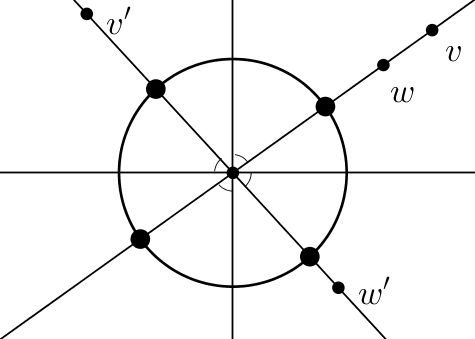
\includegraphics[scale=0.3]{circ}
\end{figure}

Luego $v\sim w\Leftrightarrow f(v)\mathcal{R}f(w)\Leftrightarrow\pi'(f(v))=\pi'(f(w))$. Entonces, tenemos el siguiente diagrama
\[
\begin{tikzcd}
\R^2\setminus\{0\} \ar[r, "f"]\arrow[d,"\pi "] & S^1 \arrow[r,"g"]\arrow[d,"\pi' "] & \R^2\setminus\{0\}\arrow[d,"\pi "]\\
\Pro_1\R \arrow[r, dashrightarrow, "\tilde{f} "] & S^1/\mathcal{R}\arrow[r, dashrightarrow, "\tilde{g} "] & \Pro_1\R
\end{tikzcd}
\]
Las aplicaciones $\tilde{f}([v])=[f(v)]$ y $\tilde{g}([x])=[g(x)]$ son continuas por la proposición \ref{149}. Además
\begin{gather*}
\tilde{g}(\tilde{f}([v]))=[g(f(v))]=\left[\frac{v}{\norm{v}}\right]=[v]\Rightarrow\tilde{g}\circ\tilde{f}=Id\\
\tilde{f}(\tilde{g}([v]))=[f(g(v))]=[v]\Rightarrow\tilde{f}\circ\tilde{g}=Id
\end{gather*}
Por todo ello, $\tilde{f}$ es homeomorfismo.\\
Tenemos entonces que todos los puntos de la parte de abajo de $S^1$ tienen un único representante arriba (salvo los extremos $(0,1)$ y $(0,-1)$, que representan el mismo punto de $\Pro_1\R$), así que si los identificamos $S^1/\mathcal{R}\cong S^1$.

\begin{figure}[h]
	\centering
	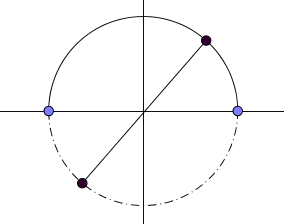
\includegraphics[scale=0.4]{s1}
\end{figure}

Para ello definimos $h\func{S^1}{S^1}$ de modo que si $e^{i\theta}\in S^1$ con $0\leq\theta\leq 2\pi$ entonces $h(e^{i\theta})=e^{i2\theta}$. Observemos lo siguiente:
\begin{gather*}
e^{i2\theta}=e^{i2\psi}\Leftrightarrow\left\{\begin{array}{c}
cos(2\theta)=cos(2\psi)\\
sen(2\theta)=sen(2\psi)
\end{array}\right\}\Leftrightarrow\begin{array}{c c}
\textit{o bien } & 2\theta=2\psi\Rightarrow\theta=\psi\\
\textit{o bien } & 2\theta=2\psi+2k\pi\Rightarrow\theta=\psi+\pi
\end{array}
\end{gather*}
Podemos definir entonces $\mathcal{R}_h$ de modo que dos puntos de la circunferencia están relacionados si y solo si son el mismo o son opuestos. Luego, con $\tilde{h}$ como homeomorfismo, $\Pro_1\R=S^1/\mathcal{R}\cong S^1$.\\
\item[$\boxed{\Pro_2\R}$] Análogamente al ejemplo anterior, definimos $f\func{\R^3\setminus\{0\}}{S^2}\mid f(v)=\dfrac{v}{\norm{v}}$ y $g\func{S^2}{\R^3\setminus\{0\}}\mid g(x)=x$. Tendremos pues el siguiente diagrama donde para $x,y \in S^2$, $x\mathcal{R}y\Leftrightarrow x=\pm y$
\[
\begin{tikzcd}
\R^3\setminus\{0\} \ar[r, "f"]\arrow[d,"\pi "] & S^2 \arrow[r,"g"]\arrow[d,"\pi' "] & \R^3\setminus\{0\}\arrow[d,"\pi "]\\
\Pro_2\R \arrow[r, dashrightarrow, "\tilde{f} ","\cong"'] & S^2/\mathcal{R}\arrow[r, dashrightarrow, "\tilde{g} "] & \Pro_2\R
\end{tikzcd}
\]
Además, si denotamos por $E^+$ a la semiesfera superior y sobre ella la relación $x\mathcal{R}'y\Leftrightarrow x=y$ ó $x,y\in S^1$ (el borde de la semiesfera) con la relación antipodal, se tiene un homeomorfismo

\begin{equation*}
\Pro_2\R\overset{\tilde{f}}{\cong} S^2/\mathcal{R}\overset{(1)}{\cong} E^+/\mathcal{R}'
\end{equation*}

Para encontrar el homeomorfismo $(1)$ consideramos las aplicaciones $k:E^+\longhookarrow S^2$ y $h\func{S^2}{E^+}$, donde $k$ es la inclusión y $h(x,y,z)=(x,y,|z|)$. Entonces es inmediato que $\mathcal{R}'$ es compatible con $\pi\circ k$ y que $\mathcal{R}$ lo es con $\pi\circ h$, por lo que tenemos el siguiente diagrama
\[
\begin{tikzcd}
E^+ \ar[r, "k"]\arrow[d,"\pi "] & S^2 \arrow[r,"h"]\arrow[d,"\pi' "] & E^+\arrow[d,"\pi "]\\
E^+/\mathcal{R}' \arrow[r, dashrightarrow, "\tilde{k} "] & S^2/\mathcal{R}\arrow[r, dashrightarrow, "\tilde{h} "] & E^+/\mathcal{R}'
\end{tikzcd}
\]
donde $\tilde{h}$ y $\tilde{k}$ son continuas y además $\tilde{h}\circ\tilde{k}=Id$ y $\tilde{k}\circ\tilde{h}=Id$, por lo que son homeomorfismos.

En lugar de $E^+$ podemos tomar la bola cerrada $B^2$, pues ambos espacios son homeomorfos, y la relación correspondiente a $\mathcal{R}'$  sobre $B^2$,  $p\mathcal{R}''q\Leftrightarrow p=q$ ó $p,q\in S^1$ y $p=\pm q$.
Vamos ahora al caso general.\\
\item[$\boxed{\Pro_n\R}$] Tendremos en general el cociente $B^n/\sim$ con $p\sim q\Leftrightarrow p=q$ ó $p,q\in S^{n-1}$ y $p=\pm q$. De esta forma $\Pro_n\R\cong B^n/\sim$. Nótese que en el borde de la bola aparece $\Pro_{n-1}\R$.
\begin{center}
\begin{tikzpicture}[line cap=round,line join=round,>=triangle 45,x=1.0cm,y=1.0cm]
\clip(-5.4066666666666645,-2.5) rectangle (8.78,1.4);
\draw [line width=1.2pt,fill=black,fill opacity=0.1] (0.,0.) circle (1.cm);
\draw [line width=1.2pt,] (0.24565880350762515,0.9693563597868443)-- (0.12666666666666662,1.16);
\draw [line width=1.2pt,] (0.24565880350762515,0.9693563597868443)-- (0.06,0.7866666666666654);
\draw [line width=1.6pt,] (-0.24886078369838055,-0.9685392662855894)-- (-0.04666666666666665,-0.826666666666667);
\draw [line width=1.2pt,] (-0.24886078369838055,-0.9685392662855894)-- (-0.06,-1.1733333333333333);
\draw (0.23333333333333325,1.4) node[anchor=north west] {$\Pro_1\mathbb{R}$};
\draw (-0.32666666666666655,0.2933333333333324) node[anchor=north west] {$\Pro_2\mathbb{R}$};
\draw (-1.5,0.25) node[anchor=north west] {$a$};
\draw (1.1533333333333329,0.25) node[anchor=north west] {$a$};
\begin{scriptsize}
\draw [fill=black] (-1.,0.) circle (2.5pt);
\draw [fill=black] (1.,0.) circle (2.5pt);
\end{scriptsize}
\end{tikzpicture}
\end{center}
\end{ej}

\begin{ejer}(Importante) $\Pro_2\R$ se puede ``ver'' en  $\R^4$. Sea $f\func{S^2}{\R^4}\mid f(x,y,z)=(xy,yz,xz,x^2 +2y^2 +3z^2)$
\begin{enumerate}
\item Probar que $f(p)=f(q)\Leftrightarrow p=\pm q$.
\item Deducir que $\Pro_2\R$ es homeomorfo a un subespacio de $\R^4$.
\end{enumerate}
\begin{solucion}\
\begin{enumerate}
\item $\boxed{\Leftarrow}$ Sean $(x,y,z)=\pm(x',y',z')\Rightarrow f(x,y,z)=(xy,yz,xz,x^2 +2y^2 +3z^2)=f(x',y',z')$.\\
$\boxed{\Rightarrow}$ Para esta implicación diferenciaremos varios casos.
\begin{itemize}
\item $x,y,z\neq 0$\\
$f(x,y,z)=f(x',y',z')\Rightarrow\left\{\begin{array}{c}
xy=x'y'\\
yz=y'z'\\
xz=x'z'\\
\end{array}\right.\Rightarrow x',y',z'\neq 0$\\
Esto implica
\begin{gather*}
\frac{x}{x'}=\frac{y'}{y};\ \frac{y}{y'}=\frac{z'}{z};\\
\frac{x}{x'}=\frac{z'}{z}=\frac{y}{y'}=\frac{x'}{x}\Rightarrow x^2=(x')^2\Rightarrow x=\pm x'
\end{gather*}
Por lo que o bien
\[
x=x'\Rightarrow y=y',z=z'
\]
o bien
\[
x=-x'\Rightarrow y=-y',z=-z'
\]
\item $x=0$, $y,z\neq 0$\\
En primer lugar, como $(x,y,z)\in S^2\Rightarrow x^2+y^2+z^2=1\Rightarrow x^2+2y^2+3z^2=2+z^2$. Ahora
\begin{gather*}
f(x,y,z)=f(x',y',z')\Rightarrow\left\{\begin{array}{c}
0=xy=x'y'\\
0=xz=x'z'\\
0\neq yz=y'z'
\end{array}\right.
\end{gather*}
De las dos últimas expresiones deducimos que $x'=0$, luego
\[
2+(z')^2=2+z^2\Rightarrow z=\pm z'\Rightarrow y=\pm y'.
\]
\item $x=y=0$, $z\neq 0$\\
Como $(x,y,z)\in S^2\Rightarrow z=\pm 1$. Entonces
\begin{gather*}
xy=x'y'=0\\
yz=y'z'=0\\
xz=x'z'=0\\
0+0+3z^2=3=(x')^2+2(y')^2+3(z')^2=1+(y')^2+2(z')^2\Rightarrow 2=(y')^2+2(z')^2
\end{gather*}
Ahora bien, $z'\neq 0$ porque si lo fuera, $|y'|=\sqrt{2}>1$. Aplicando esto a las igualdades anteriores y despejando $z'$ de esta última, llegamos a que
\[
x'=0, y'=0, z'=\pm 1
\]
\end{itemize}
\item $X=f(S^2)\subseteq\R^4$ es un compacto Hausdorff y $f\func{S^2}{X}$ es sobreyectiva. Por la propiedad universal esto significa que $\tilde{f}\func{S^2/\mathcal{R}_f}{X}$ es homeomorfismo. \qed
\end{enumerate}
\end{solucion}
\end{ejer}

\begin{ejer} Probar que el cociente $\R/\mathcal{R}$ no es Hausdorff, donde $x\mathcal{R}y\Leftrightarrow x=y$ ó $x,y\in\Q$.
\begin{solucion}
$\boxed{RA}$ Sean $[x],[y]\in\R/\mathcal{R}$ con $[x]\in U$ abierto, $[y]\in V$ abierto, y $U\cap V=\emptyset$. Por definición de topología cociente, si denotamos $\pi\func{\R}{\R/\mathcal{R}}$ a la proyección canónica, entonces $\pi^{-1}(U)$ y $\pi^{-1}(V)$ son abiertos. Además, $U\cap V=\emptyset\Rightarrow \pi^{-1}(U\cap V)=\pi^{-1}(U)\cap\pi^{-1}(V)=\emptyset$. Se tiene
\begin{itemize}
\item $\pi^{-1}(U)$ abierto $\Rightarrow \exists\ q\in\Q\mid q\in\pi^{-1}(U)\Rightarrow [q]\in U$.
\item $\pi^{-1}(V)$ abierto $\Rightarrow \exists\ q'\in\Q\mid q'\in\pi^{-1}(V)\Rightarrow [q']\in V$.
\end{itemize}
Pero $[q]=[q']\in U\cap V$, con lo que hemos llegado a una contradicción. \qed
\end{solucion}
\end{ejer}

\vspace{0.2cm}

\begin{nota} Si $A\subseteq X$ y $\mathcal{R}$ es la relación $x\mathcal{R}y\Leftrightarrow x=y$ ó $x,y\in A$, se suele escribir $X/A$.
\end{nota}

\begin{ejer} Probar que $\R^2/D^2$ es homeomorfo a $\R^2$, siendo $D^2$ la bola unidad cerrada. Ayuda: usar la función $f\func{\R^2}{\R^2}$ definida a trozos como $f(D^2)=0$ y $f(x)=\dfrac{||x||-1}{||x||}x\ \forall x\in\R^2\setminus D^2$.
\end{ejer}

\newpage

\section{Modelos Topológicos}
Antes de comenzar con la clasificación de superficies es importante familiarizarse con los modelos usados para representarlas. Estos modelos son una especie de ``instrucciones"\ sobre cómo se construye la superficie. Resultan especialmente importantes cuando tratamos con superficies que no pueden ser representadas en 3 dimensiones. Veamos algunos ejemplos.

\vspace{0.4cm}

\begin{ej}[Modelo de una caja]\

\definecolor{zzttqq}{rgb}{0.6,0.2,0.}
\begin{tikzpicture}[line cap=round,line join=round,>=triangle 45,x=1.0cm,y=1.0cm]
\clip(-1.58,-2.5) rectangle (13.753333333333336,4.5);
\fill [color=zzttqq,fill=zzttqq, fill opacity=0.1](0.,0.)-- (0.,2.)--(2,2)--(4,2)--(4,4)--(6,4)--(6,2)--(8,2)--(8,0)--(6,0)--(6,-2)--(4,-2)--(4,0)--(2,0)--cycle;
\draw (0.,0.)-- (0.,2.);
\draw (0.,0.)-- (2.,0.);
\draw (2.,0.)-- (2.,2.);
\draw (0.,2.)-- (2.,2.);
\draw (2.,0.)-- (4.,0.);
\draw (4.,0.)-- (4.,2.);
\draw (2.,2.)-- (4.,2.);
\draw (4.,0.)-- (6.,0.);
\draw (6.,0.)-- (6.,2.);
\draw (4.,2.)-- (6.,2.);
\draw (6.,0.)-- (8.,0.);
\draw (8.,0.)-- (8.,2.);
\draw (6.,2.)-- (8.,2.);
\draw (4.,2.)-- (4.,4.);
\draw (4.,4.)-- (6.,4.);
\draw (6.,4.)-- (6.,2.);
\draw (4.,0.)-- (4.,-2.);
\draw (4.,-2.)-- (6.,-2.);
\draw (6.,-2.)-- (6.,0.);
\draw [->] (4.,2.) -- (4.,3.1);
\draw [->] (4.,2.) -- (3.0066666666666673,2.);
\draw [->] (4.,4.) -- (5.046666666666668,4.);
\draw [->] (6.,2.) -- (6.,3.1);
\draw [->] (6.,2.) -- (7.153333333333335,2.);
\draw [->] (6.,0.) -- (7.006666666666668,0.);
\draw [->] (6.,0.) -- (6.,-1.1666666666666674);
\draw [->] (8.,0.) -- (8.,1.0333333333333339);
\draw [->] (2.,2.) -- (0.8733333333333335,2.);
\draw [->] (0.,0.) -- (0.,1.14);
\draw [->] (2.,0.) -- (0.9,0.);
\draw [->] (4.,0.) -- (2.9666666666666672,0.);
\draw [->] (4.,0.) -- (4.,-1.153333333333334);
\draw [->] (4.,-2.) -- (5.18,-2.);
\draw (3.6066666666666674,3.2866666666666684) node[anchor=north west] {$a$};
\draw (3.0466666666666673,2.446666666666668) node[anchor=north west] {$a$};
\draw (4.886666666666668,4.446666666666669) node[anchor=north west] {$c$};
\draw (0.9266666666666669,2.46) node[anchor=north west] {$c$};
\draw (5.02,-2.02) node[anchor=north west] {$g$};
\draw (0.9533333333333335,-0.08666666666666671) node[anchor=north west] {$g$};
\draw (3.5,-0.7666666666666672) node[anchor=north west] {$f$};
\draw (3.033333333333334,-0.02) node[anchor=north west] {$f$};
\draw (6.14,3.2466666666666684) node[anchor=north west] {$b$};
\draw (6.926666666666668,2.5) node[anchor=north west] {$b$};
\draw (8.22,1.193333333333334) node[anchor=north west] {$d$};
\draw (-0.5,1.2466666666666675) node[anchor=north west] {$d$};
\draw (6.86,0.0066666666666666706) node[anchor=north west] {$e$};
\draw (6.206666666666668,-0.7933333333333338) node[anchor=north west] {$e$};
\end{tikzpicture}

\end{ej}

\begin{ej}[Plano proyectivo]\

\definecolor{qqffqq}{rgb}{0.,1.,0.}
\definecolor{zzttqq}{rgb}{0.6,0.2,0.}
\begin{tikzpicture}[line cap=round,line join=round,>=triangle 45,x=1.0cm,y=1.0cm]
\clip(-1.82,-1.1) rectangle (13.513333333333335,1.1);
\draw[fill=qqffqq, opacity=0.1](1,0) circle (1cm);
\draw [shift={(0.,0.)},color=zzttqq,fill=zzttqq,fill opacity=0.1]  (0,0) --  plot[domain=-1.3918053133444221:1.3941368213526866,variable=\t]({1.*0.3560735948210689*cos(\t r)+0.*0.3560735948210689*sin(\t r)},{0.*0.3560735948210689*cos(\t r)+1.*0.3560735948210689*sin(\t r)}) -- cycle ;
\draw [shift={(2.,0.)},color=zzttqq,fill=zzttqq,fill opacity=0.1]  (0,0) --  plot[domain=1.7474558322371072:4.533397966934215,variable=\t]({1.*0.3514841123014168*cos(\t r)+0.*0.3514841123014168*sin(\t r)},{0.*0.3514841123014168*cos(\t r)+1.*0.3514841123014168*sin(\t r)}) -- cycle ;
\draw [->] (2.4866666666666672,0.) -- (3.233333333333334,0.);
\draw [shift={(1.,0.)},line width=2.8pt,color=qqffqq]  plot[domain=3.141592653589793:3.4995746804907433,variable=\t]({1.*1.*cos(\t r)+0.*1.*sin(\t r)},{0.*1.*cos(\t r)+1.*1.*sin(\t r)});
\draw [shift={(1.,0.)},line width=2.8pt,color=qqffqq]  plot[domain=0.:0.3534072430575585,variable=\t]({1.*1.*cos(\t r)+0.*1.*sin(\t r)},{0.*1.*cos(\t r)+1.*1.*sin(\t r)});
\draw [shift={(1.,0.)},line width=1.2pt]  plot[domain=-2.783610626688843:0.,variable=\t]({1.*1.*cos(\t r)+0.*1.*sin(\t r)},{0.*1.*cos(\t r)+1.*1.*sin(\t r)});
\draw [shift={(1.,0.)},line width=1.2pt]  plot[domain=0.3534072430575585:3.141592653589793,variable=\t]({1.*0.9995039532145752*cos(\t r)+0.*0.9995039532145752*sin(\t r)},{0.*0.9995039532145752*cos(\t r)+1.*0.9995039532145752*sin(\t r)});
\draw [shift={(4.,0.)},color=zzttqq,fill=zzttqq,fill opacity=0.1]  (0,0) --  plot[domain=1.5893127288629036:4.730905382452701,variable=\t]({1.*0.360061723103754*cos(\t r)+0.*0.360061723103754*sin(\t r)},{0.*0.360061723103754*cos(\t r)+1.*0.360061723103754*sin(\t r)}) -- cycle ;
\draw [shift={(4.313333333333334,0.)},color=zzttqq,fill=zzttqq,fill opacity=0.1]  (0,0) --  plot[domain=-1.5707963267948966:1.5707963267948966,variable=\t]({1.*0.34666666666666646*cos(\t r)+0.*0.34666666666666646*sin(\t r)},{0.*0.34666666666666646*cos(\t r)+1.*0.34666666666666646*sin(\t r)}) -- cycle ;
\draw [line width=2.pt,color=qqffqq] (4.,0.)-- (3.993333333333334,0.36);
\draw [line width=2.pt,color=qqffqq] (4.313333333333334,0.)-- (4.313333333333334,-0.34666666666666646);
\draw [->] (5.,0.) -- (6.,0.);
\draw [shift={(6.833333333333335,0.)},color=zzttqq,fill=zzttqq,fill opacity=0.1]  (0,0) --  plot[domain=1.5385494443596441:4.745709976262935,variable=\t]({1.*0.413548331180555*cos(\t r)+0.*0.413548331180555*sin(\t r)},{0.*0.413548331180555*cos(\t r)+1.*0.413548331180555*sin(\t r)}) -- cycle ;
\draw [shift={(7.153333333333335,0.)},color=zzttqq,fill=zzttqq,fill opacity=0.1]  (0,0) --  plot[domain=-1.5707963267948966:1.5707963267948966,variable=\t]({1.*0.4*cos(\t r)+0.*0.4*sin(\t r)},{0.*0.4*cos(\t r)+1.*0.4*sin(\t r)}) -- cycle ;
\draw [->] (8.,0.) -- (9.,0.);
\draw [shift={(9.726666666666668,0.)},color=zzttqq,fill=zzttqq,fill opacity=0.1]  (0,0) --  plot[domain=1.5707963267948966:4.71238898038469,variable=\t]({1.*0.38666666666666644*cos(\t r)+0.*0.38666666666666644*sin(\t r)},{0.*0.38666666666666644*cos(\t r)+1.*0.38666666666666644*sin(\t r)}) -- cycle ;
\draw [shift={(9.726666666666668,0.)},color=zzttqq,fill=zzttqq,fill opacity=0.1]  (0,0) --  plot[domain=-1.5707963267948966:1.5707963267948966,variable=\t]({1.*0.37333333333333313*cos(\t r)+0.*0.37333333333333313*sin(\t r)},{0.*0.37333333333333313*cos(\t r)+1.*0.37333333333333313*sin(\t r)}) -- cycle ;
\draw [line width=2.pt,color=qqffqq] (6.833333333333335,0.)-- (6.846666666666668,0.4133333333333331);
\draw [line width=2.pt,color=qqffqq] (7.153333333333335,0.)-- (7.153333333333335,0.4);
\draw [line width=2.pt,color=qqffqq] (9.726666666666668,0.)-- (9.726666666666668,0.38666666666666644);
\draw [->] (1.,0.9995039532145752) -- (1.2391978767398628,0.9704599570588706);
\draw [->] (1.,-1.) -- (0.779534079620795,-0.9753946780413304);
\end{tikzpicture}
\end{ej}

\newpage

\begin{ej}[Otros modelos habituales]\

\definecolor{zzttqq}{rgb}{0.6,0.2,0.}
\begin{tikzpicture}[line cap=round,line join=round,>=triangle 45,x=1.0cm,y=1.0cm]
\clip(-0.892,-4.057333333333334) rectangle (14.228,3.156);
\fill [color=zzttqq,fill=zzttqq, fill opacity=0.1](0,0)--(0,2)--(3,2)--(3,0)--cycle;
\fill [color=zzttqq,fill=zzttqq, fill opacity=0.1](5,0)--(5,2)--(8,2)--(8,0)--cycle;
\fill [color=zzttqq,fill=zzttqq, fill opacity=0.1](10,0)--(10,2)--(13,2)--(13,0)--cycle;
\fill [color=zzttqq,fill=zzttqq, fill opacity=0.1](3.3066666666666666,-0.9866666666666666)-- (0.6666666666666667,-0.96)-- (0.6666666666666667,-2.96)--(3.3066666666666666,-2.9866666666666664)--cycle;
\fill [color=zzttqq,fill=zzttqq, fill opacity=0.1](5.,-1.)-- (8.,-1.)--(8,-3)--(5,-3)--cycle;
\draw [line width=1.2pt, fill=white] (6.521333333333334,-2.017333333333333) circle (0.5054195177166078cm);
\fill [color=zzttqq,fill=zzttqq, fill opacity=0.1](9.468,-2.9906666666666673)-- (9.441333333333333,-1.0173333333333336)--(12.613333333333332,-1.0133333333333332)--(12.613333333333332,-3.0133333333333328)--cycle;
\draw [line width=1.2pt, fill=white] (11.,-2.) circle (0.4681690103180918cm);
\draw [line width=1.2pt] (0.,0.)-- (0.,2.);
\draw [line width=1.2pt] (0.,0.)-- (3.,0.);
\draw [line width=1.2pt] (0.,2.)-- (3.,2.);
\draw [line width=1.2pt] (3.,2.)-- (3.,0.);
\draw [line width=1.2pt] (5.,0.)-- (5.,2.);
\draw [line width=1.2pt] (5.,0.)-- (8.,0.);
\draw [line width=1.2pt] (8.,0.)-- (8.,2.);
\draw [line width=1.2pt] (8.,2.)-- (5.,2.);
\draw [line width=1.2pt] (10.,0.)-- (13.,0.);
\draw [line width=1.2pt] (10.,0.)-- (10.,2.);
\draw [line width=1.2pt] (13.,0.)-- (13.,2.);
\draw [line width=1.2pt] (10.,2.)-- (13.,2.);
\draw [line width=1.2pt] (3.3066666666666666,-0.9866666666666666)-- (0.6666666666666667,-0.96);
\draw [line width=1.2pt] (5.,-1.)-- (8.,-1.);
\draw [line width=1.2pt] (0.6666666666666667,-0.96)-- (0.6666666666666667,-2.96);
\draw [line width=1.2pt] (3.3066666666666666,-0.9866666666666666)-- (3.3066666666666666,-2.9866666666666664);
\draw [line width=1.2pt] (3.3066666666666666,-2.9866666666666664)-- (0.6666666666666667,-2.96);
\draw [line width=1.2pt] (5.,-1.)-- (5.,-3.);
\draw [line width=1.2pt] (5.,-3.)-- (8.,-3.);
\draw [line width=1.2pt] (8.,-1.)-- (8.,-3.);
\draw [->] (0.,0.) -- (0.,1.);
\draw [->] (3.,0.) -- (3.,1.);
\draw [->] (5.,0.) -- (5.,1.);
\draw [->] (8.,2.) -- (8.,1.);
\draw [->] (10.,0.) -- (10.,1.);
\draw [->] (10.,2.) -- (11.494666666666665,2.);
\draw [->] (13.,0.) -- (13.,1.);
\draw [->] (10.,0.) -- (11.534666666666666,0.);
\draw [->] (0.6666666666666667,-2.96) -- (0.6666666666666667,-1.96);
\draw [->] (3.3066666666666666,-2.9866666666666664) -- (3.3066666666666666,-1.9866666666666664);
\draw [->] (0.6666666666666667,-0.96) -- (2.04064,-0.9738785185185185);
\draw [->] (3.3066666666666666,-2.9866666666666664) -- (1.9937066666666667,-2.9734044444444443);
\draw [->] (5.,-3.) -- (5.,-2.);
\draw [->] (8.,-3.) -- (8.,-2.);
\draw [->] (5.,-1.) -- (6.4946666666666655,-1.);
\draw [->] (5.,-3.) -- (6.534666666666666,-3.);
\draw [line width=1.2pt] (6.521333333333334,-2.017333333333333) circle (0.5054195177166078cm);
\draw [->] (7.026666666666666,-2.0266666666666664) -- (6.965038890401267,-1.775312120387188);
\draw (-0.3853333333333338,1.1826666666666668) node[anchor=north west] {$a$};
\draw (3.268,1.116) node[anchor=north west] {$a$};
\draw (4.574666666666666,1.156) node[anchor=north west] {$a$};
\draw (8,1.156) node[anchor=north west] {$a$};
\draw (9.4,1.0893333333333335) node[anchor=north west] {$a$};
\draw (13.281333333333333,1.156) node[anchor=north west] {$a$};
\draw (11.334666666666665,2.0093333333333336) node[anchor=north west] {$b$};
\draw (11.494666666666665,0.5293333333333333) node[anchor=north west] {$b$};
\draw (2.881333333333333,-1.7773333333333339) node[anchor=north west] {$a$};
\draw (0.7,-1.7373333333333338) node[anchor=north west] {$a$};
\draw (7.654666666666666,-1.7506666666666673) node[anchor=north west] {$a$};
\draw (5.148,-1.7506666666666673) node[anchor=north west] {$a$};
\draw (1.8546666666666662,-1.004) node[anchor=north west] {$b$};
\draw (1.9746666666666663,-2.484) node[anchor=north west] {$b$};
\draw (6.468,-2.524) node[anchor=north west] {$b$};
\draw (6.374666666666666,-0.9373333333333337) node[anchor=north west] {$b$};
\draw (6.5,-1.5773333333333337) node[anchor=north west] {$c$};
\draw (0.9613333333333329,-0.01733333333333349) node[anchor=north west] {$cilindro$};
\draw (5.2,-0.01733333333333349) node[anchor=north west] {$\textit{banda de Möbius}$};
\draw (11.281333333333333,-0.084) node[anchor=north west] {$toro$};
\draw (0.6,-3.084) node[anchor=north west] {$\textit{botella de Klein}$};
\draw (7.8,-3.0306666666666673) node[anchor=north west] {$\textit{toro doble}$};
\draw [line width=1.2pt] (9.468,-2.9906666666666673)-- (9.441333333333333,-1.0173333333333336);
\draw [line width=1.2pt] (9.441333333333333,-1.0173333333333336)-- (12.613333333333332,-1.0133333333333332);
\draw [line width=1.2pt] (12.613333333333332,-1.0133333333333332)-- (12.613333333333332,-3.0133333333333328);
\draw [line width=1.2pt] (9.468,-2.9906666666666673)-- (12.613333333333332,-3.0133333333333328);
\draw [line width=1.2pt] (11.,-2.) circle (0.4681690103180918cm);
\draw [->] (9.441333333333333,-1.0173333333333336) -- (11.,-1.);
\draw [->] (9.468,-2.9906666666666673) -- (11.188102842021598,-3.0030624904540204);
\draw [->] (11.201333333333332,-1.5773333333333337) -- (11.001275660142683,-1.5318327276352801);
\draw [->] (9.468,-2.9906666666666673) -- (9.452685046558335,-1.8573601119834466);
\draw [->] (12.613333333333332,-3.0133333333333328) -- (12.613333333333332,-1.964);
\draw (11.,-1.6) node[anchor=north west] {$c$};
\draw (10.868,-0.9773333333333337) node[anchor=north west] {$d$};
\draw (10.881333333333332,-2.5) node[anchor=north west] {$d$};
\draw (9.588,-1.764) node[anchor=north west] {$e$};
\draw (12.1,-1.7506666666666673) node[anchor=north west] {$e$};
\end{tikzpicture}

\end{ej}

\begin{ej} Distintos modelos pueden representar el mismo objeto.

\begin{tikzpicture}[line cap=round,line join=round,>=triangle 45,x=1.0cm,y=1.0cm]
\clip(-0.2,-1.2) rectangle (15.133333333333335,1.2);
\draw(2.,0.) circle (1.cm);
\draw(4.,0.) circle (1.cm);
\draw(7.,0.) circle (1.cm);
\draw(7.5,0.) circle (0.5cm);
\draw(10.,0.) circle (0.68cm);
\draw(11.7,0.) circle (0.6782329983125326cm);
\draw (3.133333333333334,0.22) node[anchor=north west] {$p$};
\draw (8.,0.15333333333333343) node[anchor=north west] {$p$};
\draw (10.253333333333334,0.22) node[anchor=north west] {$p$};
\draw (11.146666666666667,0.23333333333333348) node[anchor=north west] {$p$};
\draw (5.3,0.2466666666666668) node[anchor=north west] {$\cong$};
\draw (8.653333333333334,0.14) node[anchor=north west] {$\cong$};
\begin{scriptsize}
\draw [fill=black] (3.,0.) circle (1.5pt);
\draw [fill=black] (10.68,0.) circle (1.5pt);
\draw [fill=black] (11.021767001687467,0.) circle (1.5pt);
\draw [fill=black] (8.,0.) circle (1.5pt);
\end{scriptsize}
\end{tikzpicture}

\end{ej}

\section{Acciones de Grupos}

Dado que buena parte de esta asignatura está dedicada a presentar la topología algebraica, es necesario introducir también el concepto de acción de un grupo sobre un espacio topológico. Antes de definirlo comencemos con un ejemplo sencillo. Consideremos $\R$ y $\Z$. Fijado $z\in\Z$ podemos construir la aplicación $x\in\R\mapsto x+z\in\R$. Si la generalizamos de modo que a cada par $(n,x)\in\Z\times\R$ se le haga corresponder $x+n\in\R$ diremos que $\Z$ \emph{actúa} sobre $\R$. Nótese que $(n,x+m)$ tiene la misma imagen que $(n+m,x)$ para todo $n,m\in\Z$ y $x\in\R$. Pasemos ya a la definición formal.

\begin{defi} Sea $G$ un grupo discreto y sea $X$ un espacio topológico. Se llama \textbf{acción} de $G$ sobre $X$ a cualquier aplicación 
\begin{align*}
f&\func{G\times X}{X}\\
&\quad (g,x)\mapsto f(g,x):=gx\ \text{(notaci\'on)}
\end{align*}
cumpliendo las siguientes propiedades:
\begin{enumerate}
\item $1x=x$, donde $1$ denota el elemento neutro de $G$.
\item $\forall g,h\in G\ g(hx)=(gh)x$.
\item La aplicación $f_g\func{X}{X}$ definida como $f_g(x)=gx$ es continua $\forall g\in G$. 
\end{enumerate}

\end{defi}

\begin{nota}
La noción general de acción de grupo no requiere la última propiedad, pero aquí se está exigiendo por tratarse de espacios topológicos. En cualquier caso es habitual exigirle que sea un morfismo de la categoría correspondiente.
\end{nota}

\begin{prop}
La relación generada por $x\sim gx\ \forall x\in X, \forall g\in G$ es de equivalencia. Al cociente por esta relación se lo llama \textbf{espacio de órbitas} de la acción de $G$ en $X$, denotado como $X/G$, y las clases de equivalencia se llaman \textbf{órbitas}.
\end{prop}

\begin{defi} Dado $x\in X$, los elementos de $g\in G$ tales que $gx=x$ constituyen el \textbf{grupo de isotropía} de $x$.
\end{defi}
\begin{ejer} Comprobar que efectivamente el grupo de isotropía es un grupo.
\end{ejer}

\begin{defi} Si la acción de $G$ no tiene puntos fijos, esto es, $\not\exists x\in X\mid gx=x\ \forall g\in G$, se dice que es \textbf{libre}.
\end{defi}

\begin{ej} $\R/\Z\cong S^1$ y la acción es libre. El grupo de isotropía de todo elemento de $\R$ es $\{0\}$.
\end{ej}

\begin{ej} Sean $\R^2$ y $\Z_4$. Definimos la acción $ax$ como dar un giro de $a\frac{\pi}{2}$. En este caso $\R^2/\Z_4\cong CS^1$ abierto por abajo (o bien, el cono infinito).
\end{ej}

\end{document} 